\begin{figure}[hbtp]
\centering
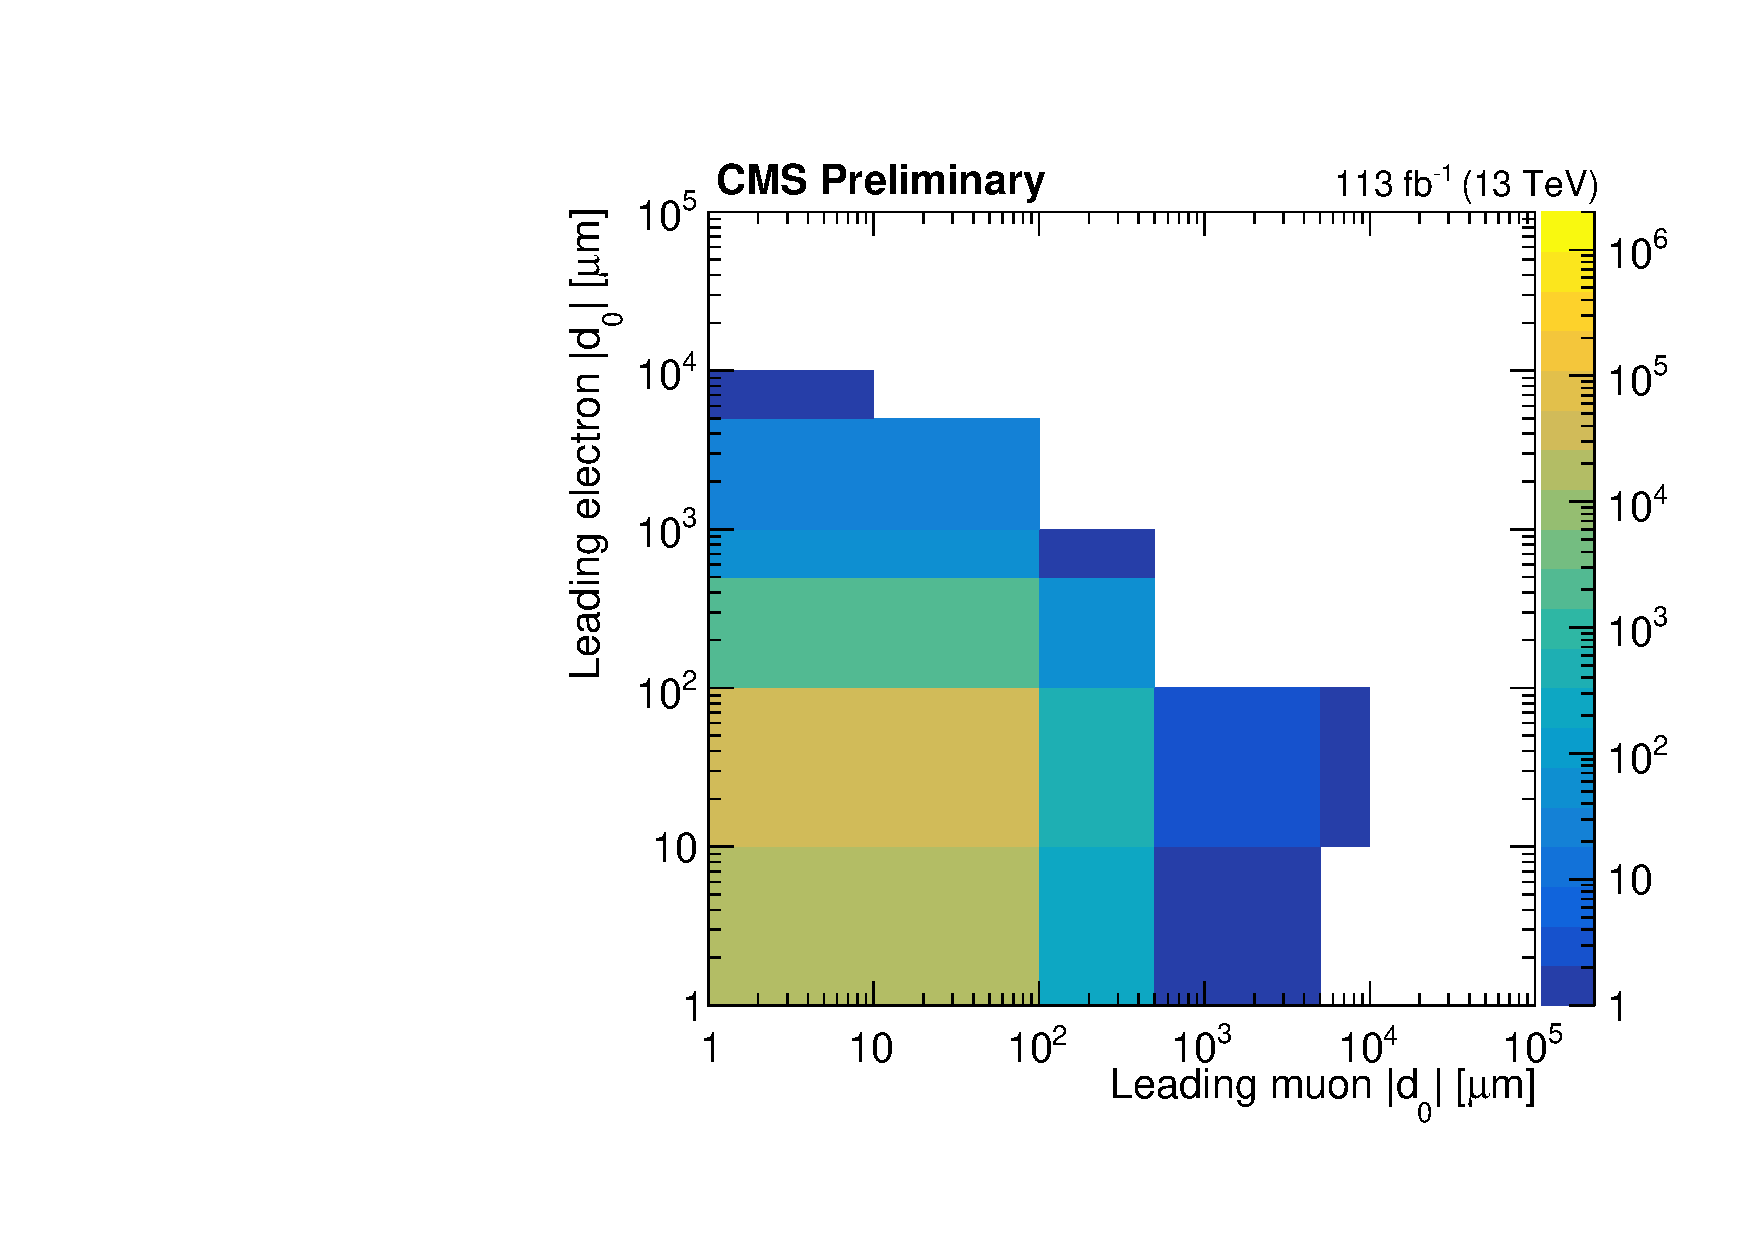
\includegraphics[width=0.32\textwidth]{figures/results/d0vsd0_emu_CMSPreliminary.pdf}
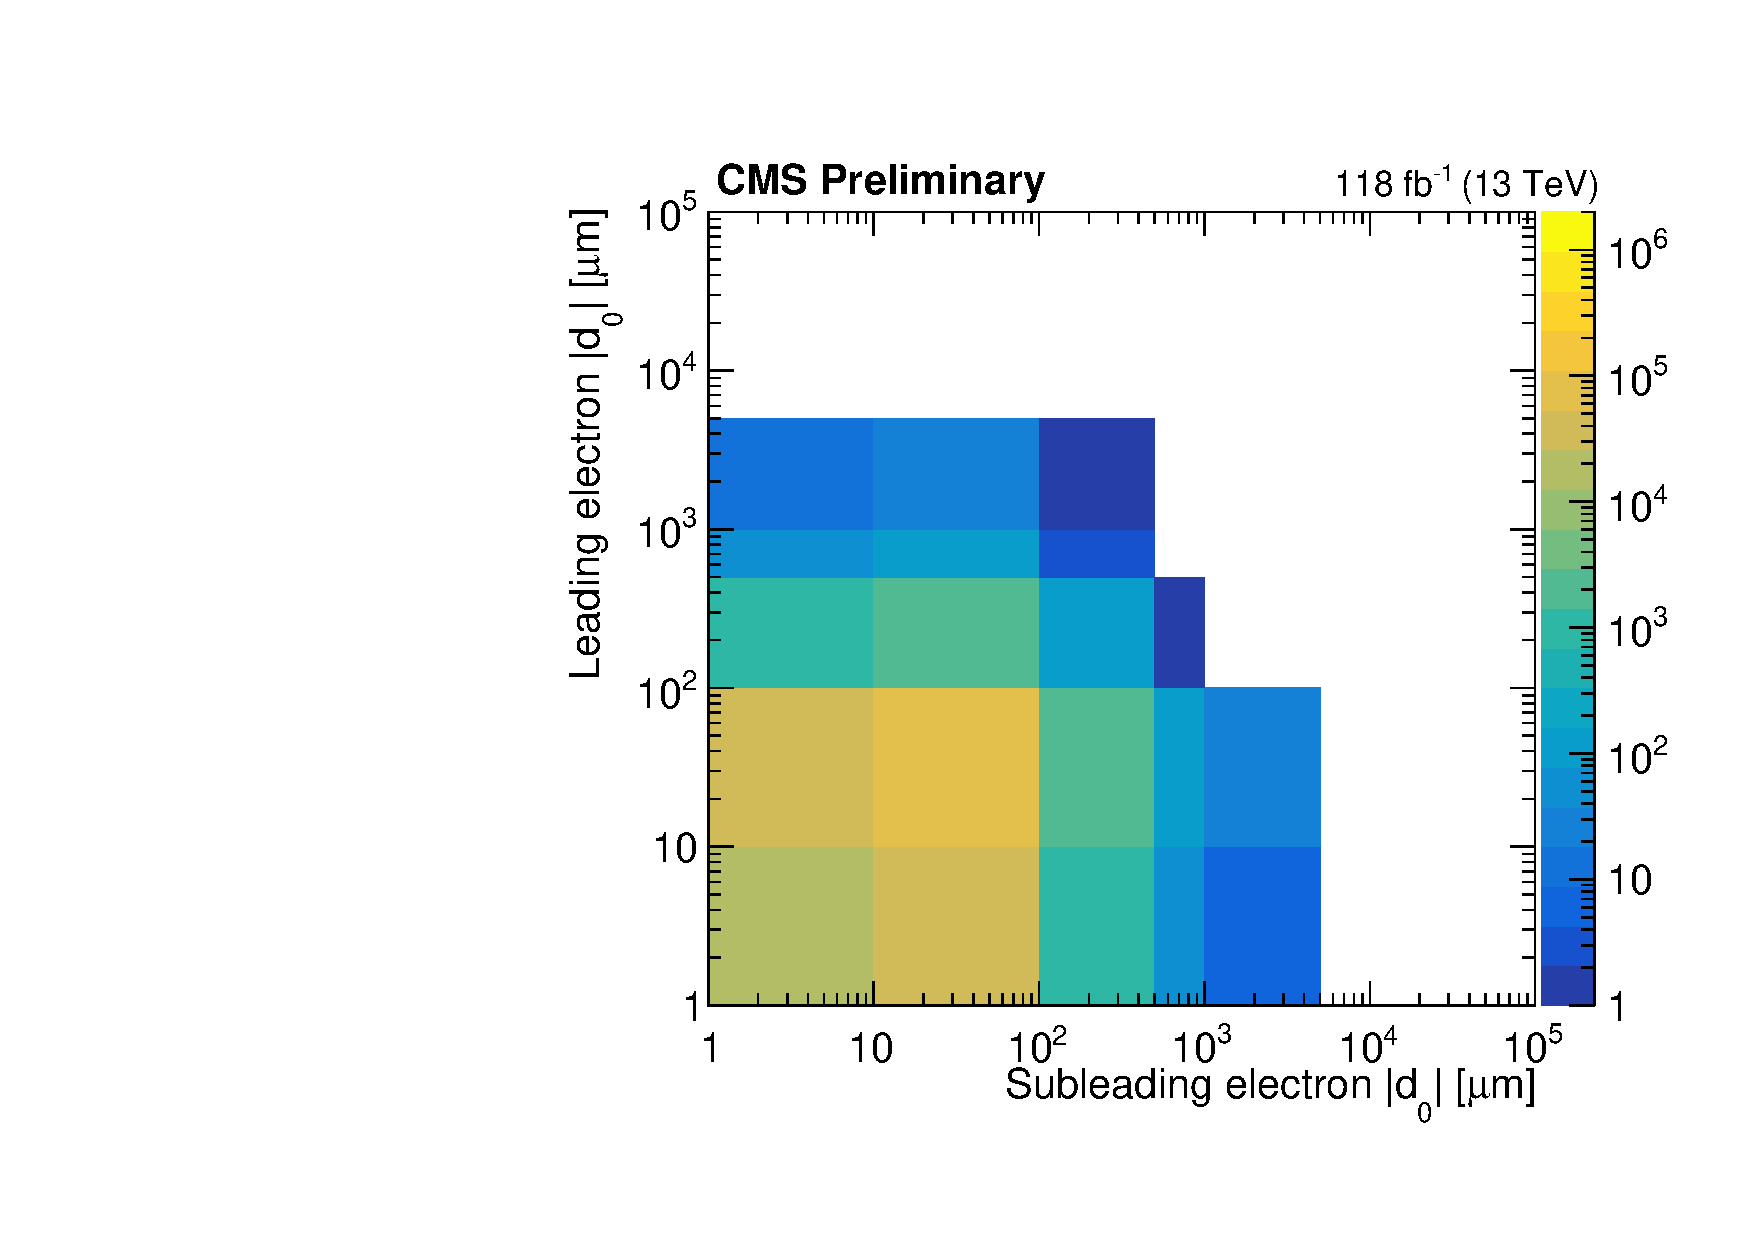
\includegraphics[width=0.32\textwidth]{figures/results/d0vsd0_ee_CMSPreliminary.pdf}
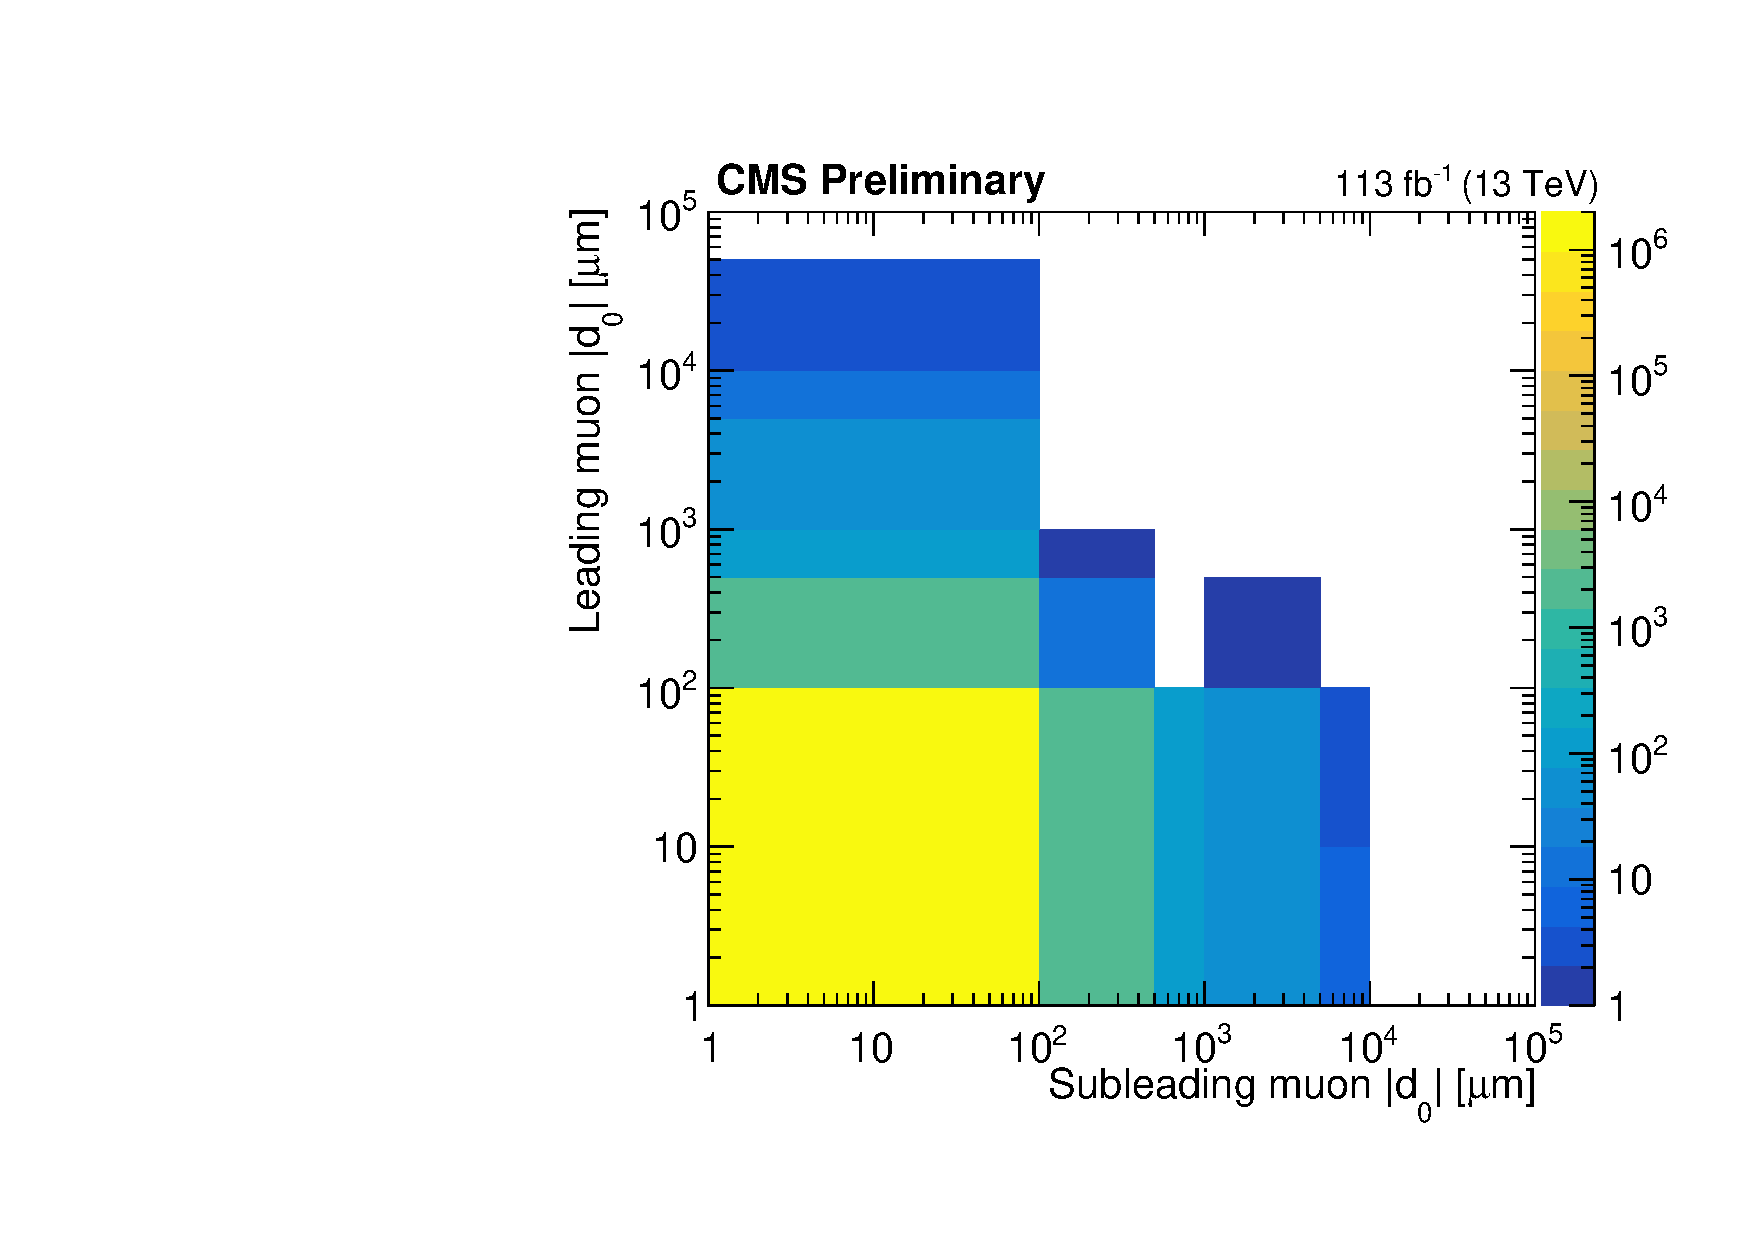
\includegraphics[width=0.32\textwidth]{figures/results/d0vsd0_mumu_CMSPreliminary.pdf}
\caption{
Two-dimensional distributions of \ada and \adb, for the events in data that pass the $\Pe\Pgm$ (left), $\Pe\Pe$ (middle), and $\Pgm\Pgm$ (right) preselection. If a \ad value is less than unity, it is set to unity in order to plot in log scale. The inclusive signal region covers the region between 100\mum and 10\cm in each \ad variable shown.
}
\label{d0_d0_data}
\end{figure}

\begin{figure}[hbtp]
\centering
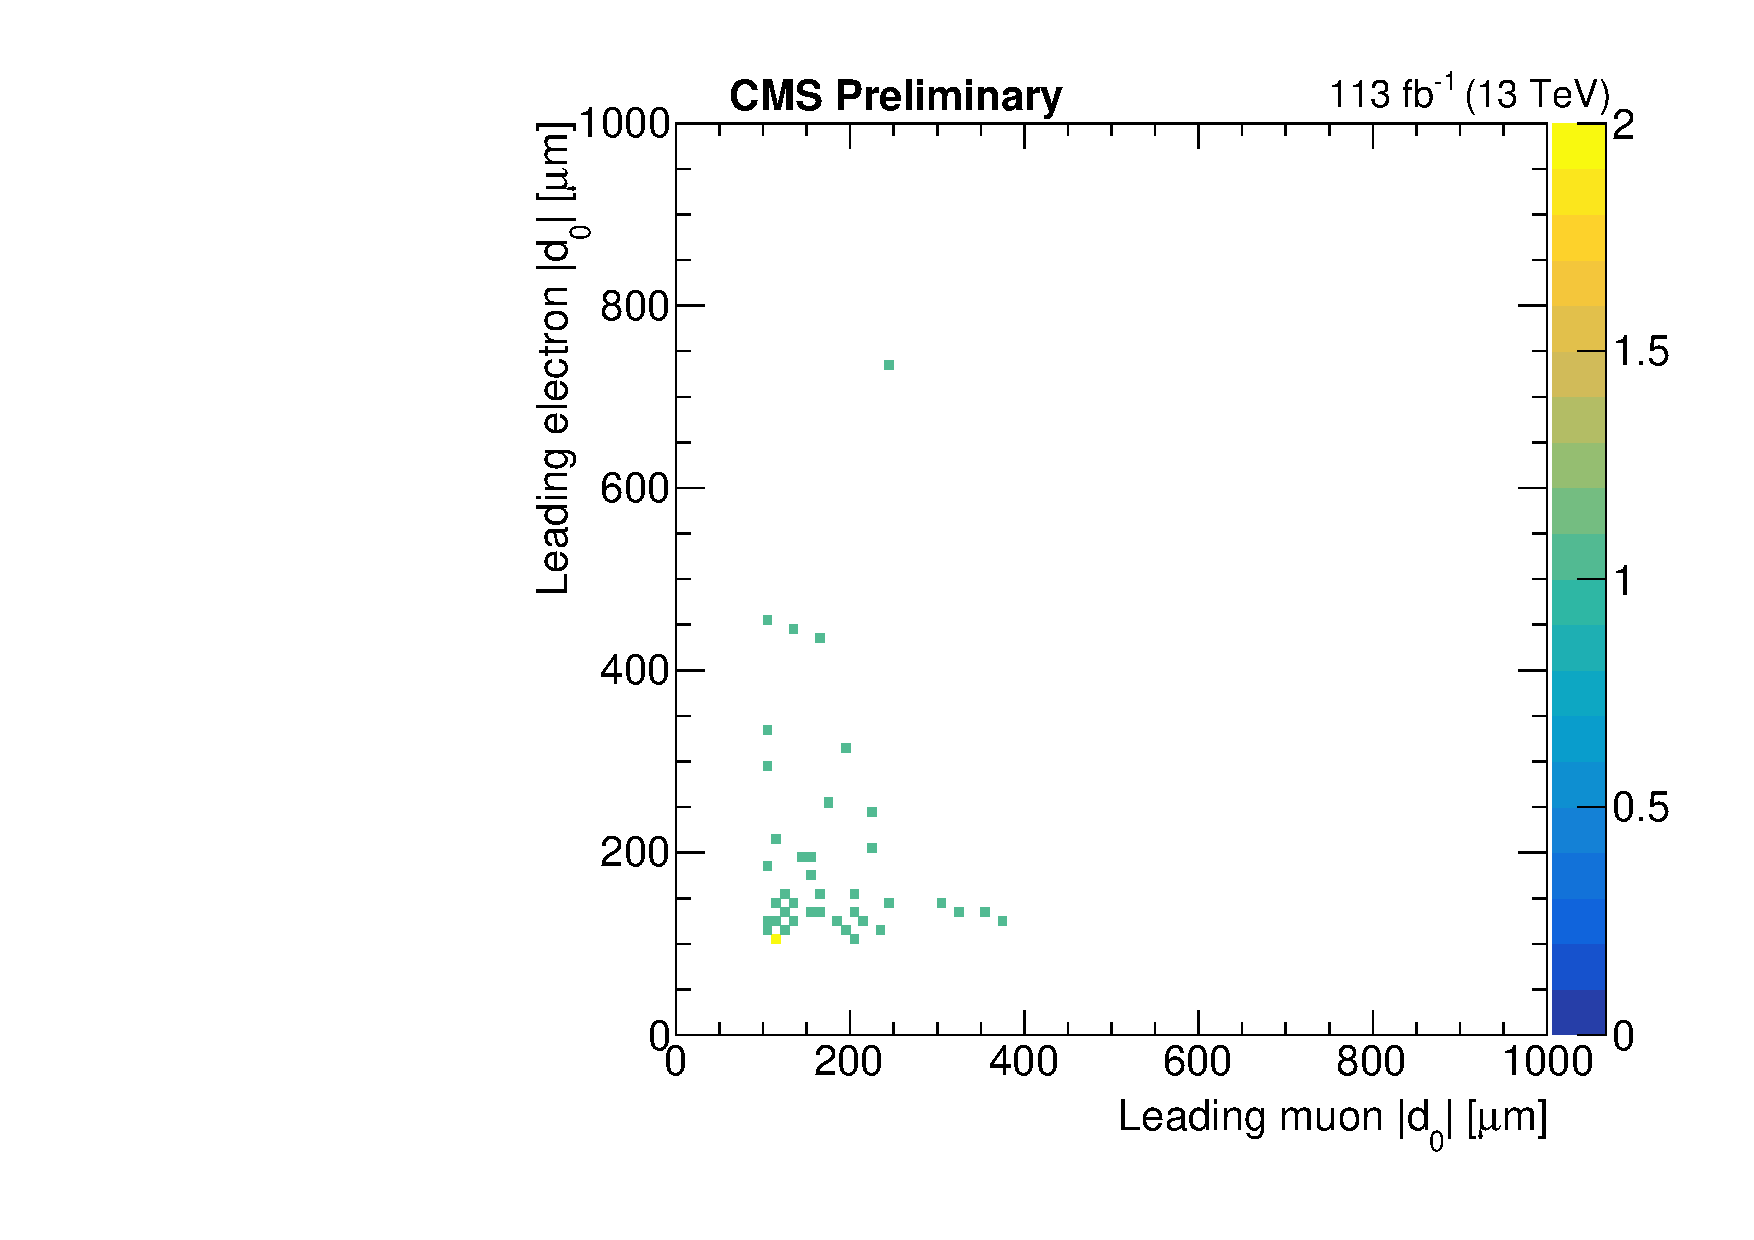
\includegraphics[width=0.31\textwidth]{figures/results/electronAbsD0[0]_vs_muonAbsD0[0]_1000um.pdf}
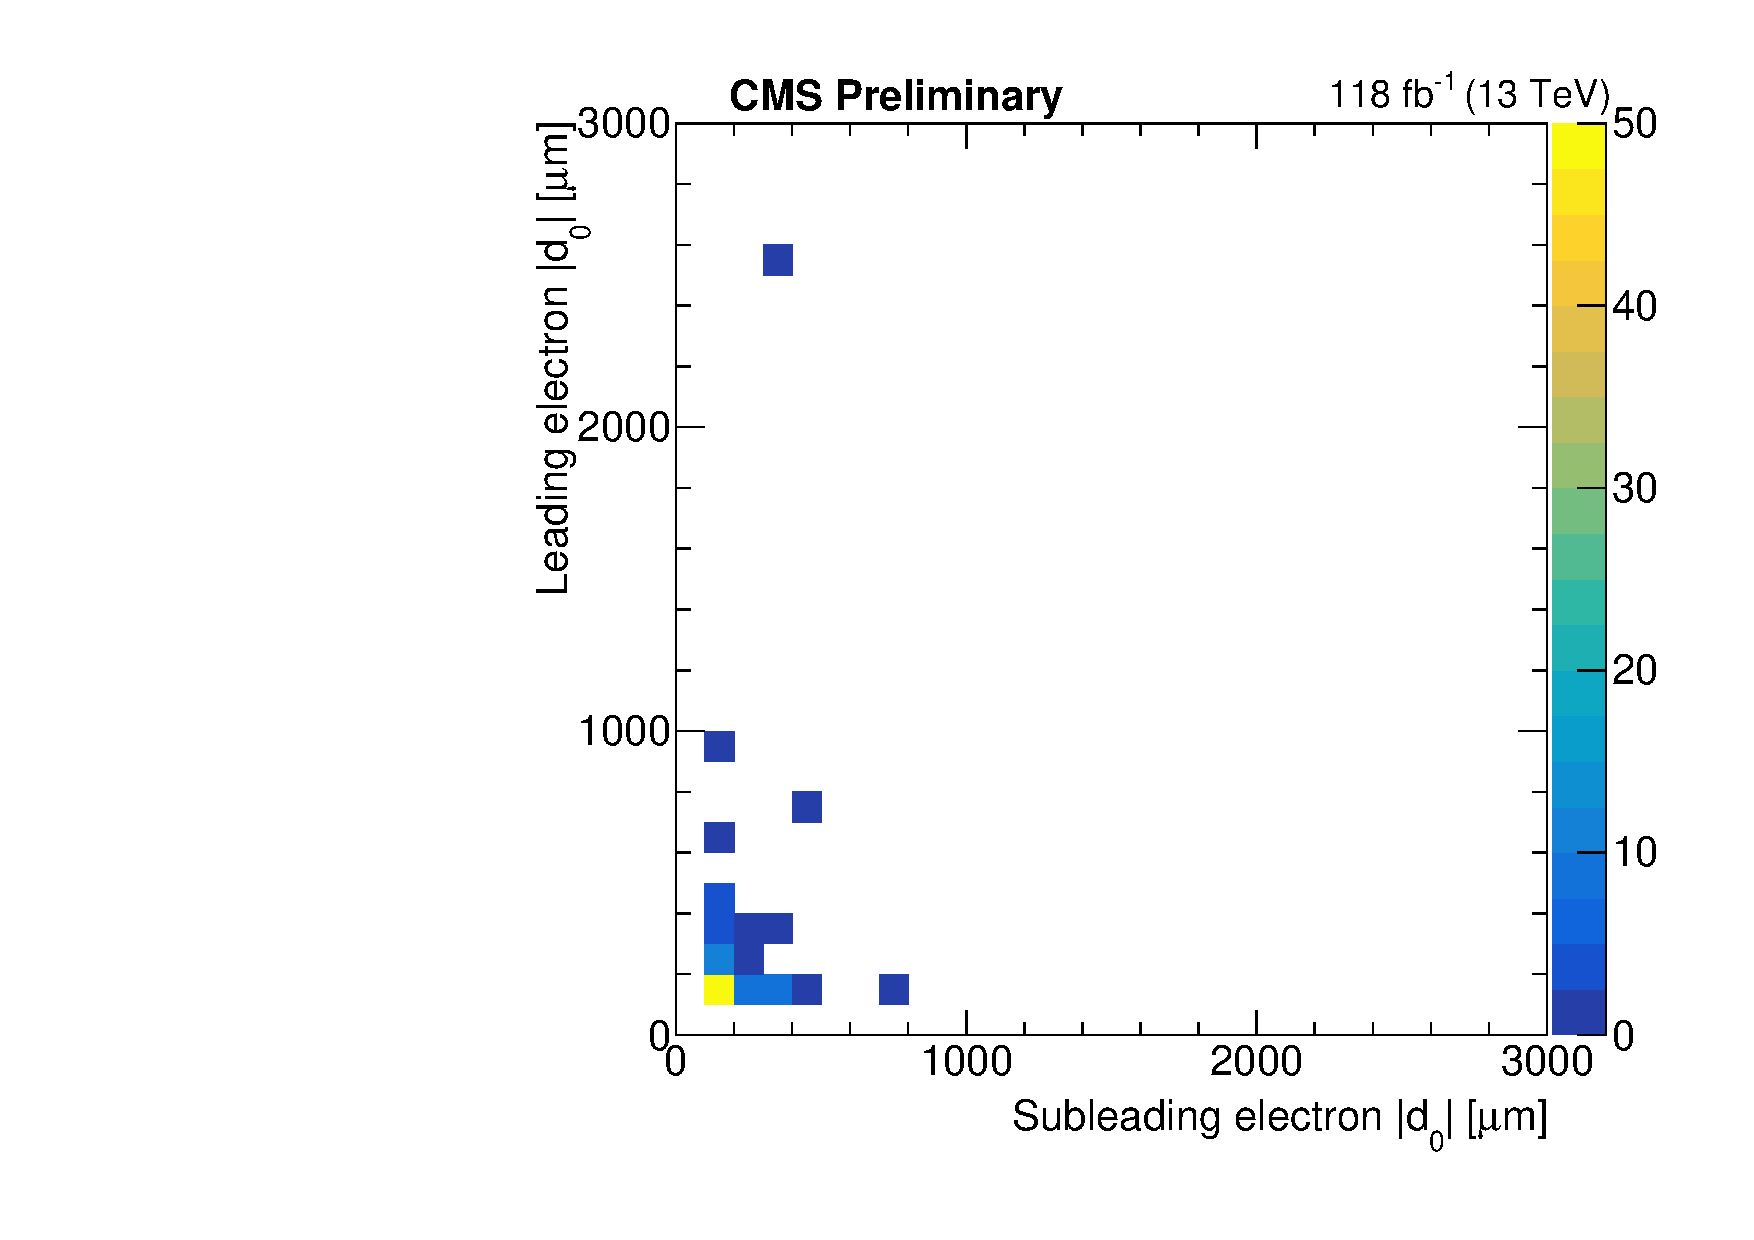
\includegraphics[width=0.31\textwidth]{figures/results/electronAbsD0[0]_vs_electronAbsD0[1]_10000um.pdf}
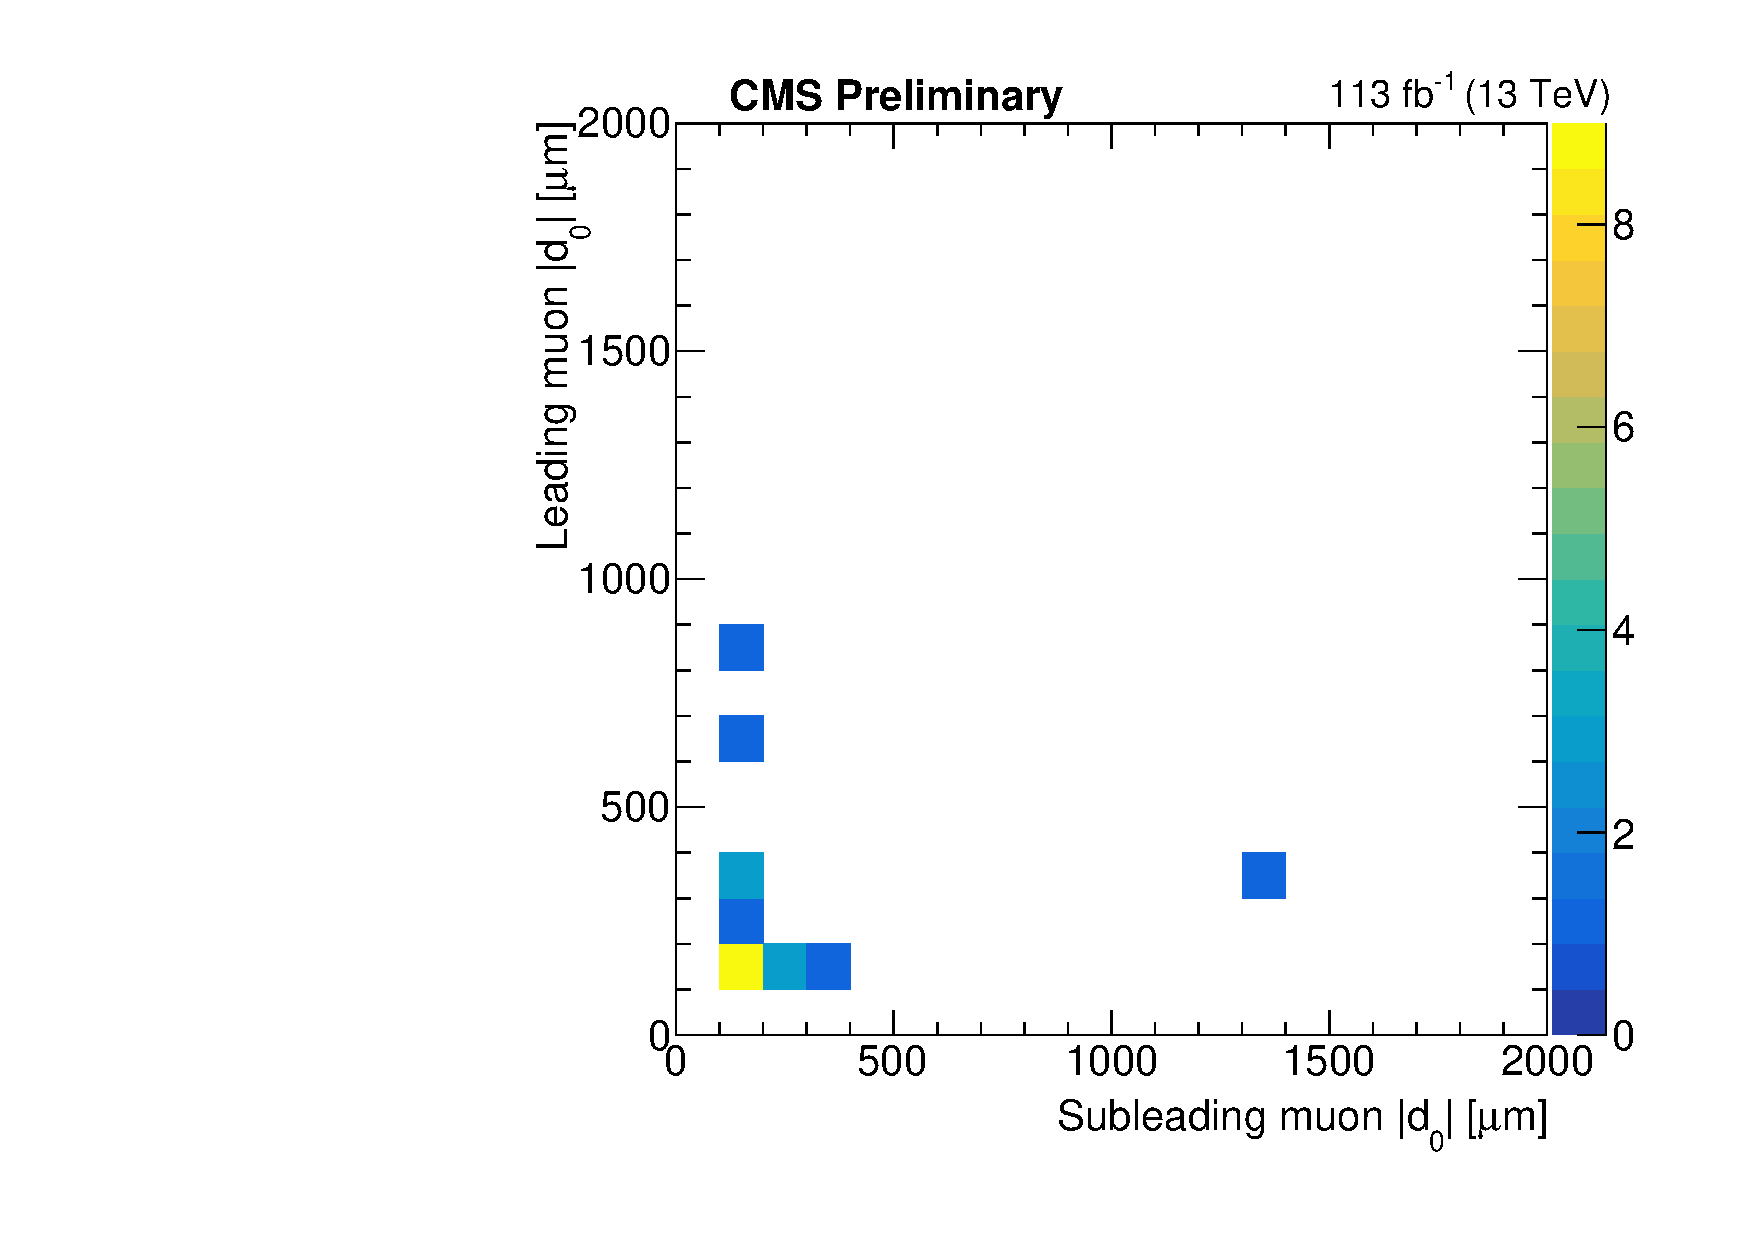
\includegraphics[width=0.31\textwidth]{figures/results/muonAbsD0[0]_vs_muonAbsD0[1]_10000um.pdf}
\caption{
Two-dimensional distributions of \ada and \adb, for data events in the inclusive SR in the $\Pe\Pgm$ (left), $\Pe\Pe$ (middle), and $\Pgm\Pgm$ (right) channels.
}
\label{d0_d0_sr_data}
\end{figure}

\begin{figure}[hbtp]
\centering
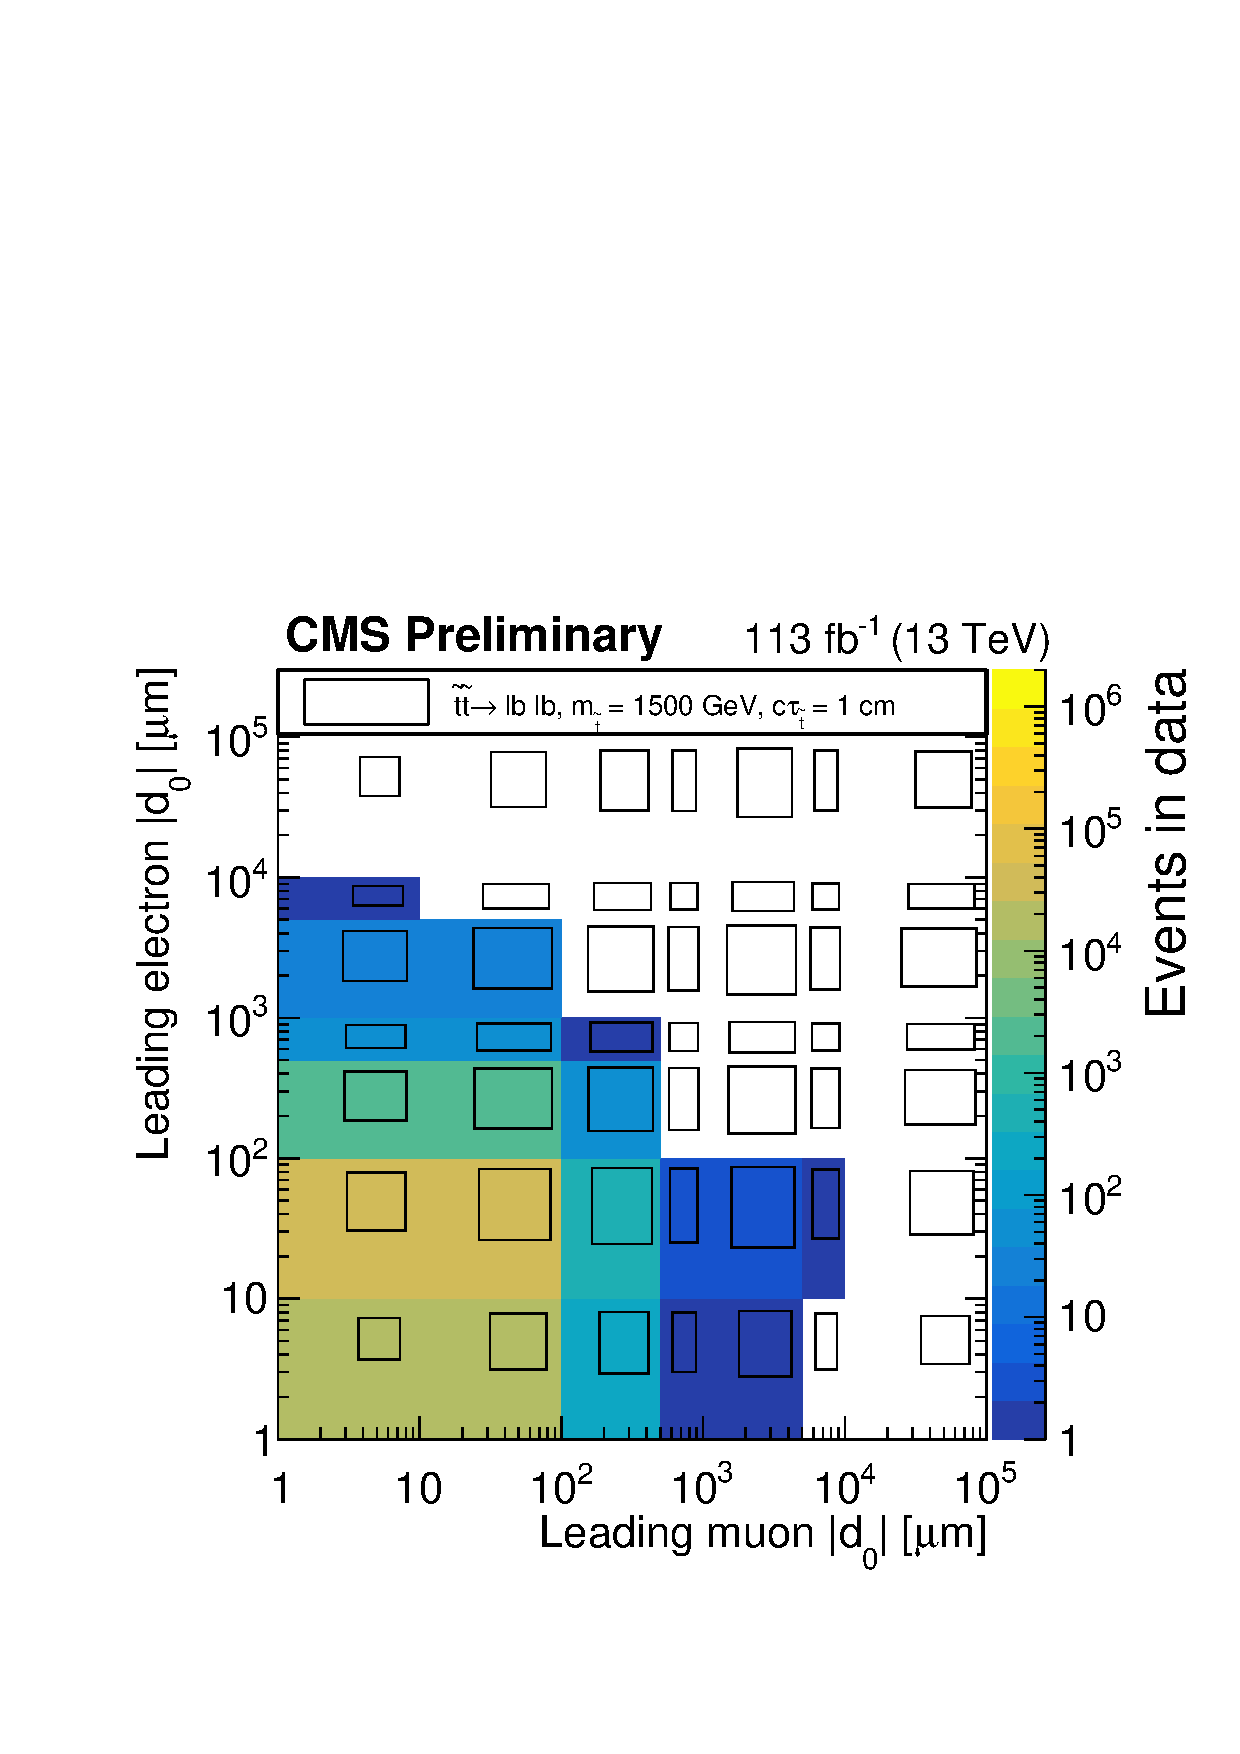
\includegraphics[width=0.6\textwidth]{figures/results/d0vsd0_emu_withSignal_CMSPreliminary.pdf}
\caption{
The two-dimensional distribution of the leading electron and leading muon \ad, for the events in data (colors) and signal (black boxes) that pass the $\Pe\Pgm$ preselection. The size of the black boxes are proportional to the size of the bin content. If a \ad value is less than unity, it is set to unity in order to plot in log scale. The inclusive signal region covers the region between 100\mum and 10\cm in each \ad variable shown.
}
\label{d0_d0_sr_data_and_signal}
\end{figure}